\documentclass[../main.tex]{subfiles}
\begin{document}
\chapter{单变量线性回归}
% Linear Regression with One Variable
\section{模型表示}
% Model Representation
\subsection{符号}
% Symbols
\begin{itemize}
    \item \(m\) 代表训练集中实例的数量
    \item \(x\) 代表特征/输入变量
    \item \(y\) 代表目标变量/输出变量
    \item \((x,y)\) 代表训练集中的实例
    \item \(({{x}^{(i)}},{{y}^{(i)}})\)代表第\(i\) 个观察实例
    \item \(h\) 代表学习算法的解决方案或函数也称为假设(\textbf{hypothesis},不是很贴切,但确实是ML中的术语)
\end{itemize}


\section{代价函数}
% Cost Function
\subsection{以直线拟合为例}
若假设函数为\(h_θ(x^{(i)}) = θ_0+θ_1x\),那么为了衡量\textbf{建模误差}(\textbf{modeling error}),提出了代价函数(\textbf{Cost Function})

\begin{figure}[H]
    \centering
    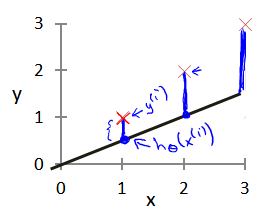
\includegraphics{./img/2.1误差.png}
    \caption{蓝线部分即此模型的误差}
\end{figure}
考虑到样本集的误差累计和数学上的含义,采取 \(J(θ_0,θ_1) = \frac{1}{2m}\sum\limits_{i=1}^m ( h_{θ}(x^{(i)})-y^{(i)} )^{2}\)作为Cost Function,算法的目标就是让误差最小,即 \(\underset{θ_0, θ_1}{\text{minimize}} J(θ_0, θ_1)\)。

最后,一共有这么几样东西:
\begin{itemize}
    \item Hypothesis:\[h_θ(x^{(i)}) = θ_0+θ_1x\]
    \item Parameters:\[θ_0,θ_1\]
    \item Cost Function:\[J(θ_0,θ_1) = \frac{1}{2m}\sum\limits_{i=1}^m ( h_{θ}(x^{(i)})-y^{(i)} )^{2}\]
    \item Goal:\[\min\limits_{θ_0, θ_1}J(θ_0, θ_1)\]
\end{itemize}


借助3D图形或Contour Map能更好的理解。

\section{代价函数的直观理解一}
\section{代价函数的直观理解二}

\section{梯度下降}
% Gradient descent
梯度下降背后的思想是:开始时我们随机选择一个参数的组合,计算代价函数,然后我们寻找下一个能让代价函数值下降最多的参数组合。我们持续这么做直到到到一个局部最小值(\textbf{local minimum}),因为我们并没有尝试完所有的参数组合,所以不能确定我们得到的局部最小值是否便是全局最小值(\textbf{global minimum}),选择不同的初始参数组合,可能会找到不同的局部最小值。
\begin{algorithm}[H]
    \caption{批量梯度下降(\textbf{batch gradient descent})}
    init \(θ_0, θ_1← 0\)\;
    \While{not convergence}{
        \(θ_j ← θ_j - α\frac{∂}{∂θ_j}J(θ_0,θ_1)\) (j=0,1)\;
    }
\end{algorithm}
其中\(α\)是学习率(\textbf{earning rate}),与偏导数值共同决定步长。另一个需要注意的地方是,\(j=0, j\),batch gradient descent算法要求同时更新两个参数(也有不同步更新的算法):\\
\begin{algorithm}[H]
    \textbf{正确的代码}:\\
    \(temp0 ← θ_0 - α\frac{∂}{∂θ_0}J(θ_0,θ_1)\)\;
    \(temp1 ← θ_1 - α\frac{∂}{∂θ_1}J(θ_0,θ_1)\)\;
    \(θ_0 ← temp0\)\;
    \(θ_1 ← temp1\)\;
    {\bfseries\color{red}错误的代码}:\\
    \(θ_0 ← θ_0 - α\frac{∂}{∂θ_0}J(θ_0,θ_1)\)\;
    \(θ_1 ← θ_1 - α\frac{∂}{∂θ_1}J(θ_0,θ_1)\)\;
\end{algorithm}

\section{梯度下降的直观理解}
若仅有一个参数,即\(J\)是二次函数,对应的是算法是:\(θ ← θ - α\frac{d}{dθ}J(θ)\),首先负号表示了\(θ\)的调节方向(最终变化于导数的正负共同决定),导数表示了增长率且J沿该方向增长最快(偏导数同理,参考梯度的意义)。
\paragraph{偏导数影响步长}在坡度较陡的地方偏导数绝对值比较大,反之,在坡度较缓的地方偏导数绝对值比较小(如接近极点处),因而不需动态改变\(α\),通过偏导数就能调节步长。
\paragraph{关于\(α\)}如果太小了,每次的步长太小,需要更多步才能到达局部最优点,会很慢,因为它会一点点挪动;弱国太大了,最糟糕的情况是越过最优点且\textit{新的位置偏导数绝对值更大},在一次次的更新中会远离最优点。
\paragraph{局部最优点和全局最优点}首先从一个初始参数开始移动,最终找到的不一定是全局最优点。若初始参数即处于导数为零处(极大或极小),则算法立即停止。在当前的情况中bowl shape函数的局部最优点等于全局最优点。

\section{梯度下降的线性回归}
对之前的线性回归问题运用梯度下降法,关键在于求出代价函数的偏导数,即:
\(j=0\)时,\(\frac{∂}{∂θ_0}J(θ_0,θ_1) = \frac{1}{m}\sum\limits_{i=1}^m(h_θ(x^{(i)})-y^{(i)})\)\\
\(j=1\)时,\(\frac{∂}{∂θ_1}J(θ_0,θ_1) = \frac{1}{m}\sum\limits_{i=1}^m(h_θ(x^{(i)})-y^{(i)})·x^{(i)}\)

\begin{remark}
    恰好2被约去
\end{remark}

还有一种正规方程\textbf{normal equations}方法,在数据量较大的情况下,梯度下降法比正规方程要更适用一些。


\end{document}